\chapter{Hybrid Situational Awareness}

\begin{figure}[htbp]
   \centering
   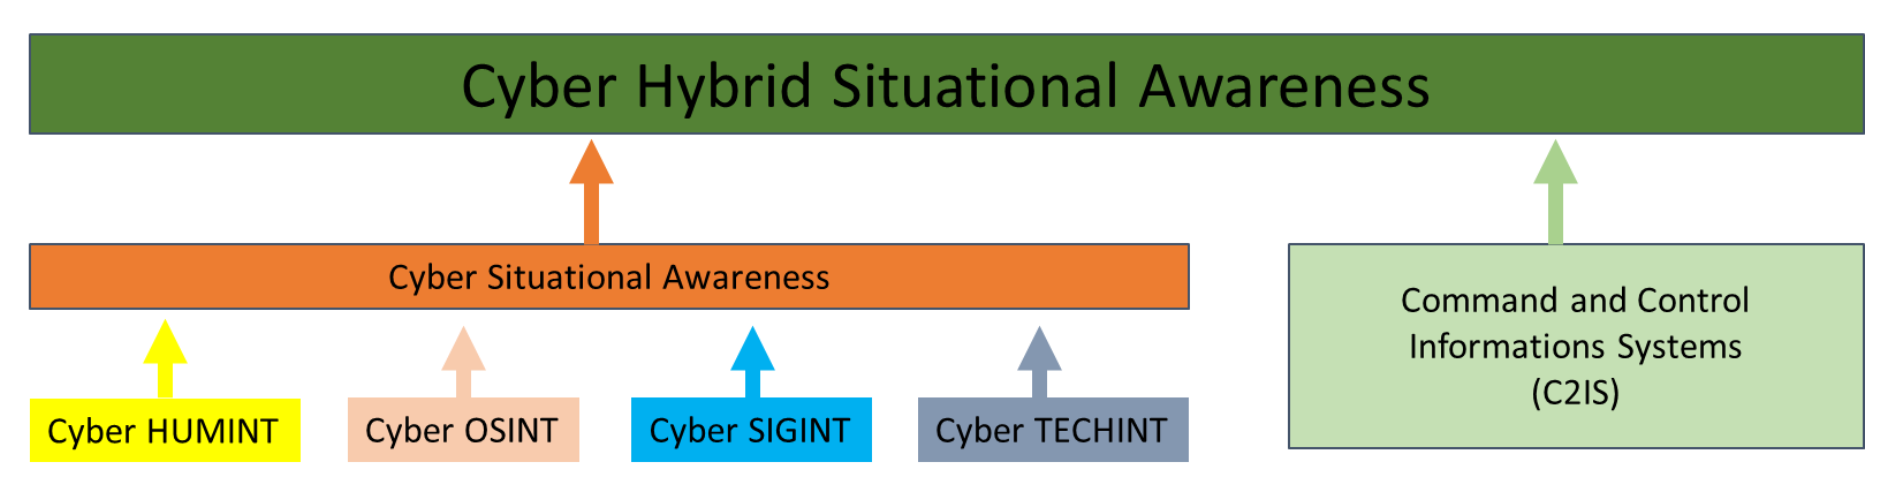
\includegraphics{images/06/CHSA.png}
   \caption{Cyber Hybrid Situational Awareness}
   \label{fig:06/CHSA}
\end{figure}

\section{Introducción}
The cybersecurity decision makers will be able to jointly perceive the situation of physical world
and cyber space domains as a unique decision making domain, as any decision taken in one
domain affects the other three.

The main ideas to generate hybrid situational awareness are:
\begin{itemize}
	\item Events in cyberspace (incidents, attacks…) produce effects in real-kinetic world, tan could affect to
course of operations and mission development
	\item Events in physical world could produce effects in cyberspace, for instance a physical attack to a
command post or to a electric grid infraestructure
	\item Cyberspace operations and kinetic operations are dependent
	\item Hybrid situational awareness is a fusion of cyber and physical situational awareness
\end{itemize}

Cada componente fisico tiene un componente ciber, y entonces lo que pasa en el mundo fisico afecta al mundo ciber y viceversa.
La Conciencia Situacional híbrida es la fusión de la CS física y la CS ciber.

\begin{figure}[htbp]
   \centering
   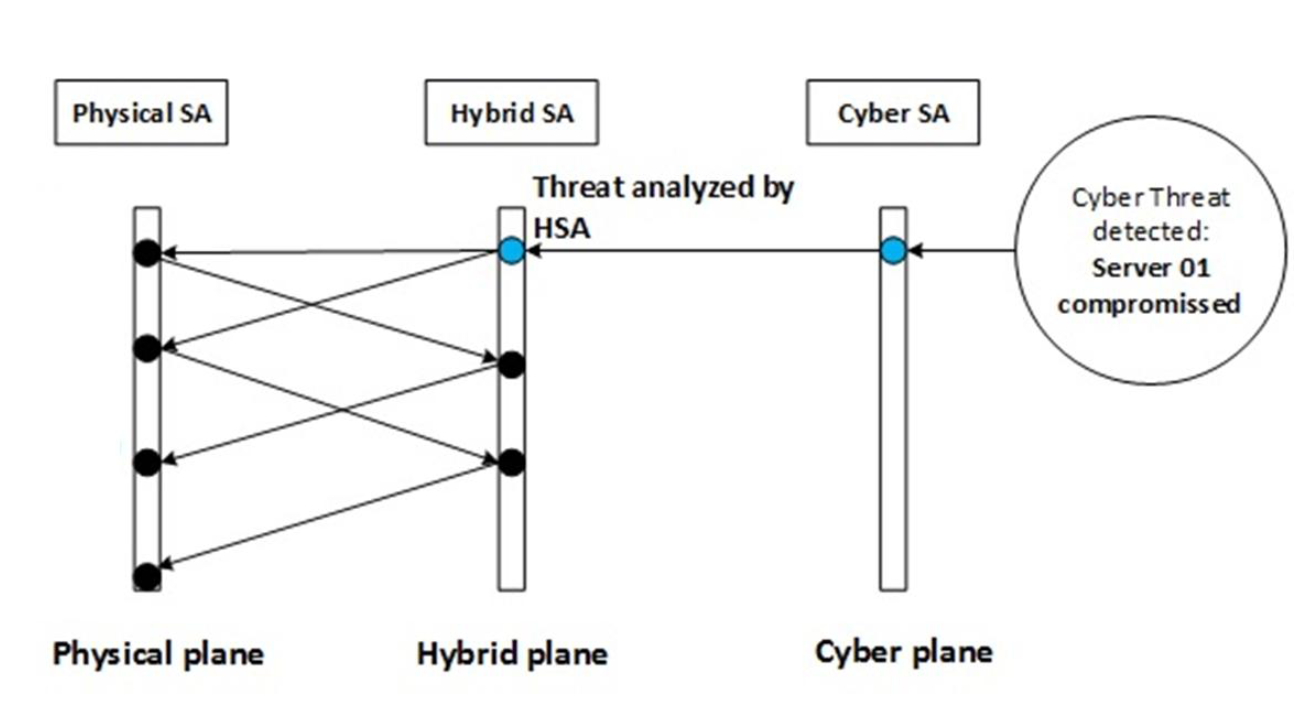
\includegraphics{images/06/cyberevent.png}
   \caption{Example of Cyber event which produces an effect in the physical world}
   \label{fig:06/cyberevent}
\end{figure}